\documentclass[dvipdfmx]{beamer}
\usepackage{amsmath, amssymb, bm, graphicx, multicol}
\usepackage{luatexja}
\usepackage{physics}
\usepackage{mathrsfs}
\usepackage{multirow}
\usepackage{float}
\usepackage{url}
\usepackage{type1cm}
\usepackage{here}

\title{量子ドット内の電子状態の数値計算}
\subtitle{~ ハイブリッドポテンシャルによる解析と差分法 ~}
\author{}
\date{}

\begin{document}

\frame{\titlepage}

\begin{frame}{目次}
\begin{enumerate}
  \item 本演習の目的
  \item 量子ドット
  \item 仮定と近似
  \item 実空間差分法
  \item 計算結果
\end{enumerate}
\end{frame}

\begin{frame}{1. 本演習の目的}
本演習では、\textbf{半導体量子ドット中の電子状態}を、解析的および数値的手法を用いて解明することを目的とする。\\

対象は、\textbf{InSb材料により形成された円形の2次元量子ドット}であり、電子はこの中に閉じ込められ、ポテンシャル井戸内でエネルギー準位が離散化される。

\begin{figure}[H]
\centering
\includegraphics[width=0.4\textwidth]{images/ドット.png}
\caption{InSb 量子ドット構造}
\end{figure}
\end{frame}

\begin{frame}{2. 量子ドット}
量子ドットは、電子の量子力学的性質を顕著に示す\textbf{人工的な原子様構造}である。\\

特徴:
\begin{itemize}
  \item \textbf{電子数を1個単位で制御}可能
  \item \textbf{波動性が顕著になるサイズ(10〜100 nm)}
\end{itemize}

応用:
\begin{itemize}
  \item 単一電子トランジスタ、量子ビット
  \item 発光素子やレーザー
\end{itemize}

\begin{figure}[H]
\centering
\includegraphics[width=0.3\textwidth]{images/量子ドット.png}
\caption{量子ドット}
\end{figure}
\end{frame}

\begin{frame}{3. 本演習で用いる仮定と近似}
\begin{itemize}
  \item \textbf{ハイブリッドポテンシャルの導入}:調和振動子と円筒壁の組合せ
  \item \textbf{有効質量近似と有効原子単位系}:$m_r$, $\varepsilon_r$ を導入
\end{itemize}
\end{frame}

\begin{frame}{3.2 有効質量近似と有効単位系}
\begin{align*}
\left[ -\frac{\hbar^2}{2m^*} \nabla^2 + V(r,\theta) \right] \psi &= E \psi \\
\Rightarrow \left[ -\frac{1}{2} \nabla^2 + V(r,\theta) \right] \psi &= E \psi \quad (\text{有効単位系})
\end{align*}

有効ボーア半径とハートリー:
\[
a_0^* = \frac{\varepsilon_r}{m_r} \cdot a_0,\quad
E_h^* = \frac{m_r}{\varepsilon_r^2} \cdot E_h
\]
\end{frame}

\begin{frame}{3.3 ハイブリッドポテンシャルの導入}
\[
V(r) =
\begin{cases}
\frac{1}{2} m^* \omega^2 r^2 & (r < R) \\
\infty & (r \geq R)
\end{cases}
\]

\begin{figure}[H]
\centering
\includegraphics[width=0.4\textwidth]{images/三種盛り.png}
\caption{量子ドットのポテンシャル}
\end{figure}
\end{frame}

\begin{frame}{4. 実空間差分法とは}
空間を格子に分割し、中心差分近似により2階微分を行う:

\[
\frac{d^2 \psi}{dx^2} \approx \frac{\psi_{i+1} - 2\psi_i + \psi_{i-1}}{\Delta x^2}
\]

\begin{figure}[H]
\centering
\includegraphics[width=0.6\textwidth]{images/一次元.png}
\caption{実空間差分法}
\end{figure}
\end{frame}

\begin{frame}{2次元シュレディンガー方程式への応用}
2次元では:
\[
\nabla^2 \psi \approx \frac{\psi_{i+1,j} + \psi_{i-1,j} + \psi_{i,j+1} + \psi_{i,j-1} - 4\psi_{i,j}}{\Delta^2}
\]

\[
-\frac{1}{2\Delta^2} (\cdots) + V_{i,j} \psi_{i,j} = E \psi_{i,j}
\]

\begin{figure}[H]
\centering
\includegraphics[width=0.35\textwidth]{images/二次元.png}
\caption{格子差分化}
\end{figure}
\end{frame}

\begin{frame}{行列形式と対角化}
差分方程式は以下のように固有値問題へ:

\[
H \bm{\psi} = E \bm{\psi}
\]

(行列式省略、画像で視覚化)

\begin{figure}[H]
\centering
\includegraphics[width=0.6\textwidth]{images/アルゴリズム.png}
\caption{対角化アルゴリズム}
\end{figure}
\end{frame}

\begin{frame}{5. 計算結果 - 課題1}
異なるポテンシャルでのエネルギー準位比較:

\begin{columns}
\column{0.32\textwidth}
\includegraphics[width=\linewidth]{images/円筒準位図.png}
\centering 円筒

\column{0.32\textwidth}
\includegraphics[width=\linewidth]{images/調和準位図.png}
\centering 調和

\column{0.32\textwidth}
\includegraphics[width=\linewidth]{images/ハイブリッド準位図.png}
\centering ハイブリッド
\end{columns}
\end{frame}

\begin{frame}{5. 計算結果 - 課題2}
閉じ込め強度$\omega$の変化に対する準位構造

\begin{figure}[H]
\centering
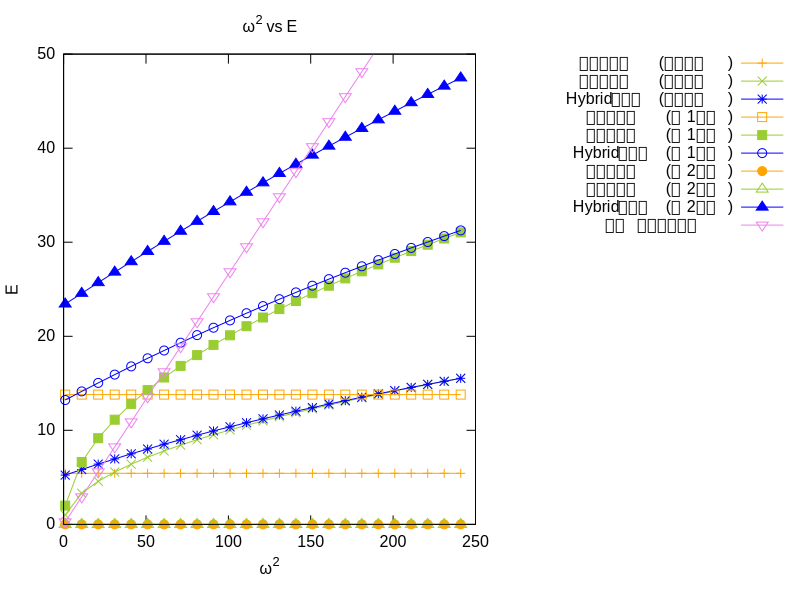
\includegraphics[width=0.7\textwidth]{images/ωE.svg}
\caption{エネルギーの閉じ込め強度依存性}
\end{figure}
\end{frame}

\end{document}
